
%%%%%%%%%%%%%%%%%%%%%%% file typeinst.tex %%%%%%%%%%%%%%%%%%%%%%%%%
%
% This is the LaTeX source for the instructions to authors using
% the LaTeX document class 'llncs.cls' for contributions to
% the Lecture Notes in Computer Sciences series.
% http://www.springer.com/lncs       Springer Heidelberg 2006/05/04
%
% It may be used as a template for your own input - copy it
% to a new file with a new name and use it as the basis
% for your article.
%
% NB: the document class 'llncs' has its own and detailed documentation, see
% ftp://ftp.springer.de/data/pubftp/pub/tex/latex/llncs/latex2e/llncsdoc.pdf
%
%%%%%%%%%%%%%%%%%%%%%%%%%%%%%%%%%%%%%%%%%%%%%%%%%%%%%%%%%%%%%%%%%%%


\documentclass[runningheads,a4paper]{llncs}
\usepackage[utf8]{inputenc}
\usepackage{amssymb}
\setcounter{tocdepth}{3}
\usepackage{graphicx}
\usepackage{listings}

\usepackage{url}
\urldef{\mailsa}\path|{alfred.hofmann, ursula.barth, ingrid.haas, frank.holzwarth,|
\urldef{\mailsb}\path|anna.kramer, leonie.kunz, christine.reiss, nicole.sator,|
\urldef{\mailsc}\path|erika.siebert-cole, peter.strasser, lncs}@springer.com|    
\newcommand{\keywords}[1]{\par\addvspace\baselineskip
\noindent\keywordname\enspace\ignorespaces#1}

\begin{document}

\mainmatter  % start of an individual contribution

% first the title is needed
\title{Resolução e Elaboração de jogos KenKen implementado em Prolog}

% a short form should be given in case it is too long for the running head
\titlerunning{Resolução/Elaboração de Jogos KenKen}

% the name(s) of the author(s) follow(s) next
%
% NB: Chinese authors should write their first names(s) in front of
% their surnames. This ensures that the names appear correctly in
% the running heads and the author index.
%
\author{Diogo Pinto ei11120
\and Wilson Oliveira ei11085}
%
\authorrunning{Resolução/Elaboração de Jogos KenKen}
% (feature abused for this document to repeat the title also on left hand pages)

% the affiliations are given next; don't give your e-mail address
% unless you accept that it will be published
\institute{FEUP-PLOG, Turma 3MIEIC06, Grupo 67\\
%\mailsa\\
%\mailsb\\
%\mailsc\\
\url{www.fe.up.pt}}

%
% NB: a more complex sample for affiliations and the mapping to the
% corresponding authors can be found in the file "llncs.dem"
% (search for the string "\mainmatter" where a contribution starts).
% "llncs.dem" accompanies the document class "llncs.cls".
%

\toctitle{Resolução/Elaboração de Jogos KenKen}
%\tocauthor{Authors' Instructions}
\maketitle


\begin{abstract}
O objectivo do trabalho é o desenvolvimento de um programa em prolog com a capacidade de resolver problemas do conhecido jogo de puzzle numerico \emph{KenKen}, e também a elaboração de puzzles deste jogo. Para a resolução deste problema será utilizado técnicas de programação com restrições em prolog. 
\keywords{KenKen, Prolog, Restrições, Resolução, Geração}
\end{abstract}

\newpage
\section{Introdução}

Este trabalho tinha como objectivo a utilização de programação com restrições em prolog, para a resolução de problemas de optimização ou decisão, verificando assim a eficácia deste método de programação em relação a métodos de tentativa e erro.
Para a realização deste objectivo decidimos implementar um programa capaz de resolver puzzle numéricos do conhecido jogo KenKen.
Neste artigo é possivel analisar os métodos utilizados para a resolução do problema em prolog, assim como excertos mais importantes do código implementado.


\section{Descrição do problema}
A implementação de um programa capaz de resolver puzzles numéricos do tipico jogo KenKen, um jogo similar a Sudoku, em que temos um tabuleiro NxN com números diferentes em cada linha e coluna. Este tabuleiro é subdividido em campos, para os quais é indicado uma operação matemática e um resultado. Estes campos impôem restricões no preenchimento do tabuleiro, uma vez que os números utilizados em cada campo, após a aplicação da operação matemática indicada, devem originar o resultado pedido.


Para a resolução deste problema foram utilizados métodos de programação com restricões em prolog, impondo restrições nos numeros que podem ser utilizados, verificando que não existem números repetidos por linha e coluna, e verificando que as operações matemáticas indicadas se evidenciam.

\section{Ficheiros de Dados}

\section{Variáveis de Decisão}
Para a resolução deste problema são necessárias quatro variáveis de decisão, primeiro o dominio dos números a serem utilizados no tabuleiro. Só podem ser utilizados no tabuleiro números de valor igual ou inferior ao tamanho do tabuleiro, por exemplo, se o tabuleiro for 4x4, só poderão ser utilizados números de um a quatro.
A segunda e terceira restrição são similares, deve ser verificado que não existem números repetidos, por coluna e linha.
A última restrição deve verificar que as operações matemáticas pedidas e respectivo resultado se verificam.
Fazendo a verificação destas quatro restrições estaremos a reduzir eficazmente o dominio de pesquisa de possiveis soluções.

\section{Restrições}
A implementação da restrição do dominio, é feita criando uma lista com as variáveis de dominio que irão ser preenchidas, e impondo a restrição do valor máximo a ser utilizado (\emph{SupLim}).
\noindent
\begin{verbatim}
imposeDomainConstrainInRow([cell(_, Value) | Rs], SupLim) :- 
	Value in 1..SupLim,										 					 				imposeDomainConstrainInRow(Rs, SupLim).
\end{verbatim}

A implementação da restrição de números diferentes numa linha é feita através da construção de uma lista com as variáveis de dominio, e utilizando a função .........", para adicionar esta restrição.
A restrição para as colunas é feita utilizando o mesmo predicado, mas é utilizado a função \emph{transpose} para inverter a ordem das listas que formam o tabuleiro.
\begin{verbatim}
imposeRowConstrain([], List) :- all_distinct(List).

imposeRowConstrain([cell(_, Value) | Rs], List) :- 
	append([Value], List, NewList),
	imposeRowConstrain(Rs, NewList).
\end{verbatim}

A implementação da restrição das operações matemáticas e feita construindo uma lista com as celulas que compoem um campo, e mediante a operação especificada nesse campo, é imposta a restrição.
\begin{verbatim}
imposeFieldConstrain(Board, [field(FID, Op, Res) | Fs]) :- 
	getFieldCells(FID, Board, L),
	applyOpConstrain(L, Op, Res),
	imposeFieldConstrain(Board, Fs).
\end{verbatim}

\section{Função de avaliação}
Penso que nao se aplica no nosso trabalho

\section{Estratégia de Pesquisa}
Na resolução de um tabuleiro, após a imposição das restrições é executado o \emph{labelling} com os valores por defeito, para obter a melhor solução possivel para o tabuleiro apresentado.

Na geração de um tabuleiro, após a imposição das restrições nas variáveis de dominio, o labelling é feito um número aleatório de vezes, com o objectivo de obter sempre tabuleiros diferentes e válidos para o mesmo tamanho pedido.

\section{Visualização da solução}
Os predicados de visualização são chamados automaticamente após a resolução de um tabuleiro.
Os predicados de impressão são bastante simples, fazendo uso da recursividade de prolog e de iteradores para fazer a construção do tabuleiro, e numerar as colunas e linhas, para facilitar a identificação dos campos internos do tabuleiro.
Como os campos são aleatórios, fizemos uso de carateres ascii para salientar a diferença entre campos e ao mesmo tempo tornar o tabuleiro mais apelativo. Também é impressa um lista com os detalhes dos campos (operação matemática, e resultado final) e fazendo uso da numeração do tabuleiro, a coluna e linha onde se inicia o campo, sendo facilmente identificável as restantes células desse campo.

Predicado responsável por salientar a mudança de campo no tabuleiro, entre células adjacentes na mesma linha.
\begin{verbatim}
printRow([C1]) :- 
	cell(_, Value1) = C1,  
	printNumber(Value1),
	write('||\n').

printRow([C1, C2 | Cs]) :- 
	cell(FieldID1, Value1) = C1, 
	cell(FieldID2, _Value2) = C2, 
	FieldID1 = FieldID2, 
	printNumber(Value1),
	write('|'), 
	printRow([C2 | Cs]).

printRow([C1 | Cs]) :- 
	cell(_, Value1) = C1,
	printNumber(Value1),
	write('||'), 
	printRow(Cs).
\end{verbatim}

Predicado responsável por salientar a mudança de campo no tabuleiro, entre células adjacentes na mesma coluna.
\begin{verbatim}
printHorizMidBorder([R1 | R1s], [R2 | R2s]) :- 
	cell(FieldID1, _) = R1, 
	cell(FieldID2, _) = R2, 
	FieldID1 = FieldID2, 
	write('---='), 
	printHorizMidBorder(R1s, R2s). 

printHorizMidBorder([_R1 | R1s], [_R2 | R2s]) :- 
	write('===='), 
	printHorizMidBorder(R1s, R2s).
\end{verbatim}

\begin{figure}
\centering
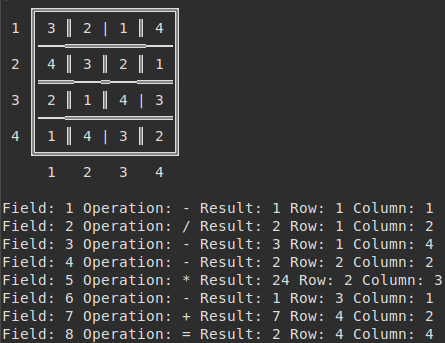
\includegraphics[height=6.2cm]{solve}
\caption{Picture of a solved board.}
\label{fig:example}
\end{figure}

\section{Resultados}

\section{Conclusões e perspectivas de desenvolvimento}
Após análise dos resultados obtidos e diferentes testes, podemos concluir que os métodos de programação com restrições se tornam mais eficazes que métodos de tentativa e erro, uma vez que limitam à priori o nível de possibilidades para a resolução do problema tornando mais eficaz a procura de uma solução válida.

\section{Bibliografia}

\begin{thebibliography}{4}

\bibitem{url} Sicstus Documentation, \url{http://sicstus.sics.se/sicstus/docs/latest/html/sicstus.html/}

\bibitem{url} Swi-Prolog Documentation, \url{http://www.swi-prolog.org/pldoc/refman/}

\end{thebibliography}

\newpage
\appendix
\section{kenken.pl}
\lstset{
language=Prolog,
numbers=left,
frame=single,
breaklines=true,
}

%\lstinputlisting{kenken.pl}

\end{document}
